\documentclass[11pt,compress,t,notes=noshow]{beamer}\usepackage[]{graphicx}\usepackage[]{color}

\makeatletter
\def\maxwidth{ %
  \ifdim\Gin@nat@width>\linewidth
    \linewidth
  \else
    \Gin@nat@width
  \fi
}
\makeatother

\definecolor{fgcolor}{rgb}{0.345, 0.345, 0.345}
\newcommand{\hlnum}[1]{\textcolor[rgb]{0.686,0.059,0.569}{#1}}%
\newcommand{\hlstr}[1]{\textcolor[rgb]{0.192,0.494,0.8}{#1}}%
\newcommand{\hlcom}[1]{\textcolor[rgb]{0.678,0.584,0.686}{\textit{#1}}}%
\newcommand{\hlopt}[1]{\textcolor[rgb]{0,0,0}{#1}}%
\newcommand{\hlstd}[1]{\textcolor[rgb]{0.345,0.345,0.345}{#1}}%
\newcommand{\hlkwa}[1]{\textcolor[rgb]{0.161,0.373,0.58}{\textbf{#1}}}%
\newcommand{\hlkwb}[1]{\textcolor[rgb]{0.69,0.353,0.396}{#1}}%
\newcommand{\hlkwc}[1]{\textcolor[rgb]{0.333,0.667,0.333}{#1}}%
\newcommand{\hlkwd}[1]{\textcolor[rgb]{0.737,0.353,0.396}{\textbf{#1}}}%
\let\hlipl\hlkwb

\usepackage{framed}
\makeatletter
\newenvironment{kframe}{%
 \def\at@end@of@kframe{}%
 \ifinner\ifhmode%
  \def\at@end@of@kframe{\end{minipage}}%
  \begin{minipage}{\columnwidth}%
 \fi\fi%
 \def\FrameCommand##1{\hskip\@totalleftmargin \hskip-\fboxsep
 \colorbox{shadecolor}{##1}\hskip-\fboxsep
     \hskip-\linewidth \hskip-\@totalleftmargin \hskip\columnwidth}%
 \MakeFramed {\advance\hsize-\width
   \@totalleftmargin\z@ \linewidth\hsize
   \@setminipage}}%
 {\par\unskip\endMakeFramed%
 \at@end@of@kframe}
\makeatother

\definecolor{shadecolor}{rgb}{.97, .97, .97}
\definecolor{messagecolor}{rgb}{0, 0, 0}
\definecolor{warningcolor}{rgb}{1, 0, 1}
\definecolor{errorcolor}{rgb}{1, 0, 0}
\definecolor{code}{rgb}{0.97, 0.96, 1.0}
\newenvironment{knitrout}{}{} % an empty environment to be redefined in TeX

\usepackage{alltt}
\usepackage[utf8]{inputenc}
\usepackage[ngerman]{babel}
\usepackage{dsfont}
\usepackage{verbatim}
\usepackage{amsmath}
\usepackage{amsfonts}
\usepackage{mathtools}
\usepackage{csquotes}
\usepackage{cmbright}
\usepackage{multirow}
\usepackage{longtable}
\usepackage{enumerate}
\usepackage[absolute,overlay]{textpos}
\usepackage{psfrag}
\usepackage{algorithm}
\usepackage{algpseudocode}
\usepackage{eqnarray}
\usepackage{bytefield}
\usepackage{animate}
\usepackage{tikz}
\usetikzlibrary{shapes,matrix,positioning,chains,arrows,shadows,decorations.pathmorphing,fit,backgrounds}
\usepackage{adjustbox}
\usepackage{colortbl}
\usepackage{tabularx} % for tables (incl. \hline)
\usepackage{arydshln} % Load after array, longtable, colortab and/or colortbl , otherwise problems with \hline in tabular env
\usepackage{etex} %increase registers for \dimenS to more than 256, otherwise we get "No room for a new \dimen"
\usepackage{graphicx}
\usepackage{booktabs} %used in epr lectures
\usepackage{bm} % bold greek letters
\usepackage{hyperref} % url citing
\usepackage{blkarray} % block arrays
\usepackage{listings} % block of code
\usepackage{xcolor} %colored math symbols
\usepackage{pgffor}
\usepackage{verbatimbox}
\usepackage{xcolor}

%some colors
\definecolor{checkgreen}{HTML}{18A126}
\definecolor{errorred}{HTML}{FF0000}
\definecolor{blockbg}{HTML}{F7F7F7}
\definecolor{gray}{HTML}{A0A0A0}

% basic latex stuff
\newcommand{\col}{\par\colorbox{code}{\parbox{\textwidth}{\theverbbox}}\par}
\newcommand{\eg}{e.\,g.\xspace} %for example
\newcommand{\ie}{i.\,e.\xspace} %that is to say...
\newcommand{\pkg}[1]{{\fontseries{b}\selectfont #1}} %fontstyle for R packages
\newcommand{\lz}{\vspace{0.5cm}} %vertical space
\newcommand{\oneliner}[1] % Oneliner for important statements
{\begin{block}{}\begin{center}\begin{Large}#1\end{Large}\end{center}\end{block}}
\def\SpAr{\quad \Rightarrow \quad}

%new environments
\newenvironment{vbframe}  %frame with breaks and verbatim
{
 \begin{frame}[containsverbatim,allowframebreaks]
}
{
\end{frame}
}

\newenvironment{vframe}  %frame with verbatim without breaks (to avoid numbering one slided frames)
{
 \begin{frame}[containsverbatim]
}
{
\end{frame}
}

\newenvironment{blocki}[1]   % itemize block
{
 \begin{block}{#1}\begin{itemize}
}
{
\end{itemize}\end{block}
}

\newenvironment{fragileframe}[2]{  %fragile frame with framebreaks
\begin{frame}[allowframebreaks, fragile, environment = fragileframe]
\frametitle{#1}
#2}
{\end{frame}}

\newcommand{\myframe}[2]{  %short for frame with framebreaks
\begin{frame}[allowframebreaks]
\frametitle{#1}
#2
\end{frame}}

\usepackage{../../style/lmu-lecture}

\let\code=\texttt
\let\proglang=\textsf

\setkeys{Gin}{width=0.9\textwidth}

\usepackage{tikz}
\usetikzlibrary{shapes,arrows,snakes, calc}

% Define block styles
\tikzstyle{decision} = [diamond, draw, text width=6em, text badly centered, node distance=4cm, inner sep=0pt]
\tikzstyle{decision2} = [diamond, draw, fill=customgreen!35, text width=6em, text badly centered, node distance=4cm, inner sep=0pt]

\tikzstyle{block} = [rectangle, draw, text width=14em, text centered, rounded corners, node distance=3cm, minimum height=4em]
\tikzstyle{line} = [draw, -latex']
\tikzstyle{cloud} = [draw, ellipse, node distance=3cm, minimum height=2em]

\title{Introduction to Deep Learning}
\author{Bernd Bischl}
\institute{Department of Statistics -- LMU Munich}
\date{WS 2021/2022}

\setbeamertemplate{frametitle}{\expandafter\uppercase\expandafter\insertframetitle}

\IfFileExists{upquote.sty}{\usepackage{upquote}}{}
\input{../../latex-math/basic-math}
\input{../../latex-math/basic-ml}
\input{../../latex-math/ml-nn}

\title{Deep Learning}
\date{}


\begin{document}
\newcommand{\titlefigure}{plots/manifold.png}
%modify picture
\newcommand{\learninggoals}{
  \item manifold hypothesis 
  656577\item manifold learning with AEs 
}



\lecturechapter{Manifold learning}
\lecture{I2DL}

\begin
{vbframe}
  \begin{itemize}
        \item \textbf{Manifold hypothesis}: 
        Data of interest lies on an embedded non-linear manifold within the higher-dimensional space.
    %    Data is concentrated around a low-dimensional \textit{manifold} or a small set of such manifolds
        %    \pause
        % \item In mathematics, a manifold is a topological space that locally resembles Euclidean space near each point 
        \item A \textbf{manifold}: 
        \begin{itemize}
        \item  is a topological space that locally resembles the Euclidean space.
        \item  in ML, more loosely refers to a connected set of points that can be approximated well by considering only a small number of dimensions. % embedded in a higher-dimensional space
        \end{itemize}
          \begin{figure}[h]
                \centering
                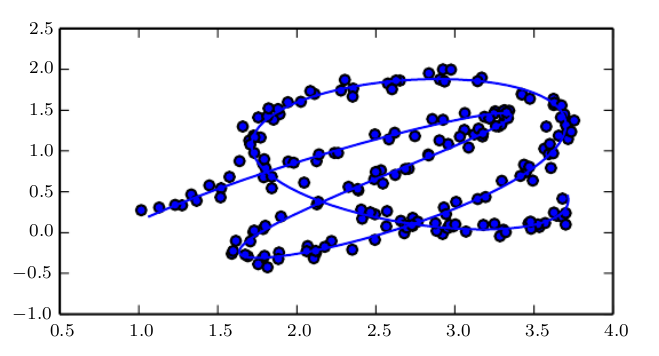
\includegraphics[width=5  cm]{plots/manifold.png}
                \caption{
                from Goodfellow et. al%Data sampled from a distribution in a 2D space that is actually concentrated near a 1D manifold.
                }
            \end{figure}
           \end{itemize}    
       \framebreak
 
\begin{itemize}
    \item An important characterization of a manifold is the set of its tangent planes.
    \item \textbf{Definition}: At a point $\xv$ on a $d$-dimensional manifold, the \textbf{tangent plane} is given by $d$ basis vectors that span the local directions of variation allowed on the manifold.
    
\end{itemize} 
        \begin{figure}[h]
            \centering
            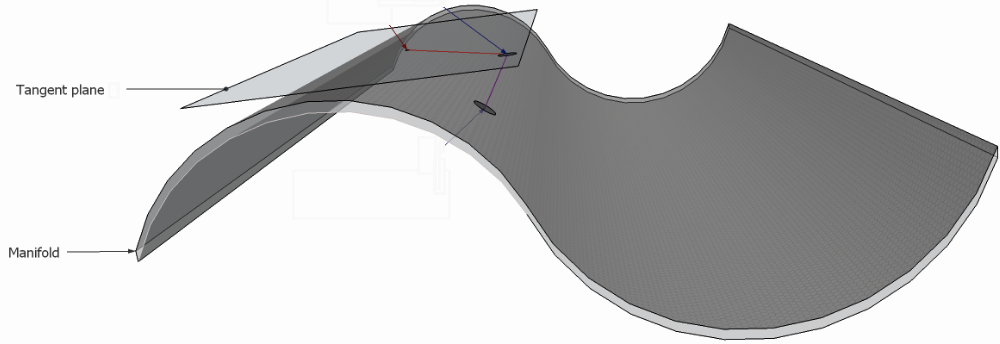
\includegraphics[width=0.8\linewidth]{plots/tangent_plane.png}
            \caption{A pictorial representation of the tangent space of a single point, \textbf{\textit{x}}, on a manifold (Goodfellow et al. (2016)).}
        \end{figure}
     
       \framebreak
       
      
        \begin{itemize}
        \item Manifold hypothesis does not need to  hold true.
        %assumption that the data lies along a low-dimensional manifold may notalways be correct
        \item In the context of AI tasks (e.g.~processing images, sound, or text) it seems to be at least approximately correct, since :
        \begin{itemize}
        \item probability distributions over images, text strings, and sounds that occur in real life are highly concentrated (randomly sampled pixel values do not look like images, randomly sampling letters is unlikely to result in a meaningful sentence).
        \item samples are connected to each other by other samples, with each sample surrounded by other highly similar samples that can be reached by applying transformations (E.g. for images: Dim or brighten the lights, move or rotate objects, change the colors of objects,  etc).
     \end{itemize}
      % TODO: add more on the manifold view ?
    \end{itemize} 

\end{vbframe}




\begin{vbframe}{Learning Manifolds with AEs}
  
    \begin{itemize}
        \item AEs training procedures involve a compromise between two forces:

            \begin{enumerate}
                \item Learning a representation $\pmb{z}$ of a training example $\xv$ such that $\xv$ can be approximately recovered from $\pmb{z}$ through a decoder.

                \item Satisfying an architectural constraint or regularization penalty.
            \end{enumerate}
   
       \item Together, they force the hidden units to capture information about the structure of the data generating distribution 
       
       \item important principle: AEs can afford to 
       represent only the variations that are needed to reconstruct training examples.
       
         \item If the data-generating distribution concentrates near a low-dimensional manifold, this yields representations that implicitly capture a local coordinate system for the manifold. 
         
         \framebreak
       
   \item Only the variations tangent to the manifold around $\xv$ need to correspond to changes in $\pmb{z}=enc(\xv)$. Hence the encoder learns a mapping from the input space to a representation space that is only sensitive to changes along the manifold directions, but that is insensitive to changes orthogonal to the manifold.  
       
       \begin{figure}
    \centering
    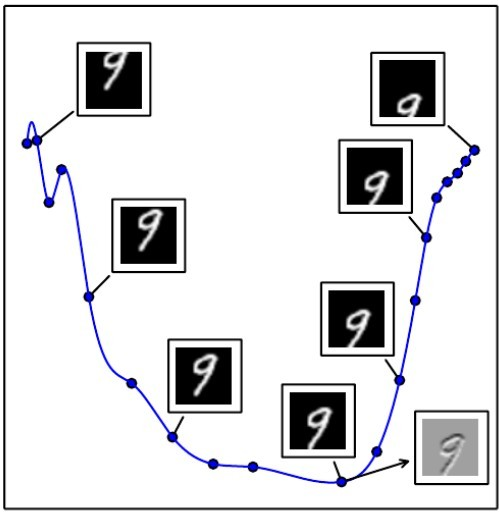
\includegraphics[width=4cm]{plots/AE-manifold.jpg}
    \caption{from Goodfellow et al. (2016) }
    \end{figure}
    
   \end{itemize}

\framebreak

    \begin{itemize}
        \item Common setting: a representation (embedding) for the points on the manifold is learned.
        \item Two different approaches
            \begin{enumerate}
                \item Non-parametric methods: learn an embedding for each training example.
                \item Learning a more general mapping for \textit{any} point in the input space.
            \end{enumerate}
        \item %Non-parametric approaches have problems with complicated manifolds\\
        AI problems can have very complicated structures that can be difficult to capture from only local interpolation.\\
            $\Rightarrow$ Motivates use of \textbf{distributed representations} and deep learning!
    \end{itemize}
\end{vbframe}




\endlecture
\end{document}